\chapter{Introducción}
\label{cap:capitulo1}
\setcounter{page}{1}

En la actualidad, los vehículos autónomos están en auge; cada vez tenemos más ejemplos de tareas realizadas por humanos que pueden ser realizadas por máquinas. Un ejemplo de ello lo encontramos en la conducción autónoma. Esta tiene el potencial de cambiar la forma en que nos movemos, aportando seguridad y confort. Si bien es cierto que aún no vemos vehículos circulando sin conductor (también por cuestiones legales), mucha de la tecnología necesaria para hacerlo ya está presente en los vehículos actuales. La conducción autónoma no solo se aplica a los vehículos que transitan las ciudades, sino que también es aplicable a muchos otros ámbitos, por ejemplo entornos industriales, de inspección o incluso de exploración, donde el vehículo se enfrenta a situaciones impredecibles y ante las que debe saber reaccionar correctamente.\\

\section{Inteligencia artificial}
\label{sec:ia}
La inteligencia artificial (o \textit{Artifical Intelligence}, (\textit{IA})) es la disciplina que intenta entender y emular el comportamiento humano. Tiene como objetivo dotar a sistemas, entre los que se encuentran los robots, de cierta inteligencia y de la capacidad de aprender. Existen multitud de ramas que parten de la inteligencia artificial, como por ejemplo, la visión artificial, el aprendizaje automático o el aprendizaje profundo. Estas técnicas permiten tomar decisiones o clasificar datos en base a una información de entrada que, en algunos casos, requiere de un entrenamiento previo mediante un conjunto grande de datos conocidos como \textit{datasets}. A través de esta información, los algoritmos que integran este tipo de técnicas obtienen lo necesario para poder inferir, por ejemplo, los objetos presentes en una imagen.\\  

\section{Visión artificial}
\label{sec:vision}
Cualquier robot necesita sensores para percibir el entorno; uno de ellos es el sensor de visión. Gracias a una cámara podemos obtener mucha información del entorno que rodea al robot y, con ello, este puede actuar en consecuencia. La cámara se presenta como el sensor más interesante que puede equipar un robot, cuentan con un tamaño y peso muy reducido, como es el caso de la cámara \textit{PiCamera} (Figura \ref{fig:picamera}), además de un coste muy bajo. Sin embargo, presenta algunas dificultades cuando nos disponemos a tratar la imagen recibida. Para procesar una imagen, y dependiendo de su resolución, es necesario un mínimo de requerimientos técnicos a nivel de \textit{hardware}, para poder conseguir un procesamiento con un nivel adecuado de fotogramas por segundo (o \textit{Frames Per Second}, \textit{FPS}), por otra parte, la imagen recibida deberá haber sido captada en un entorno con buenas condiciones lumínicas. Por ello, existen diferentes tipos de sensores electroópticos/infrarrojos (o \textit{Electro-Optical and Infrared Sensors}, \textit{EO/IR}), como por ejemplo, las cámaras de visión nocturna, donde el espectro utilizado es el conocido como infrarrojo lejano (o \textit{Far Infrared}, \textit{FIR}). Con ello se consigue resaltar en la imagen lo que realmente es necesario y se obtiene un mejor funcionamiento en situaciones de niebla.\\

\begin{figure} [h!]
	\begin{center}
		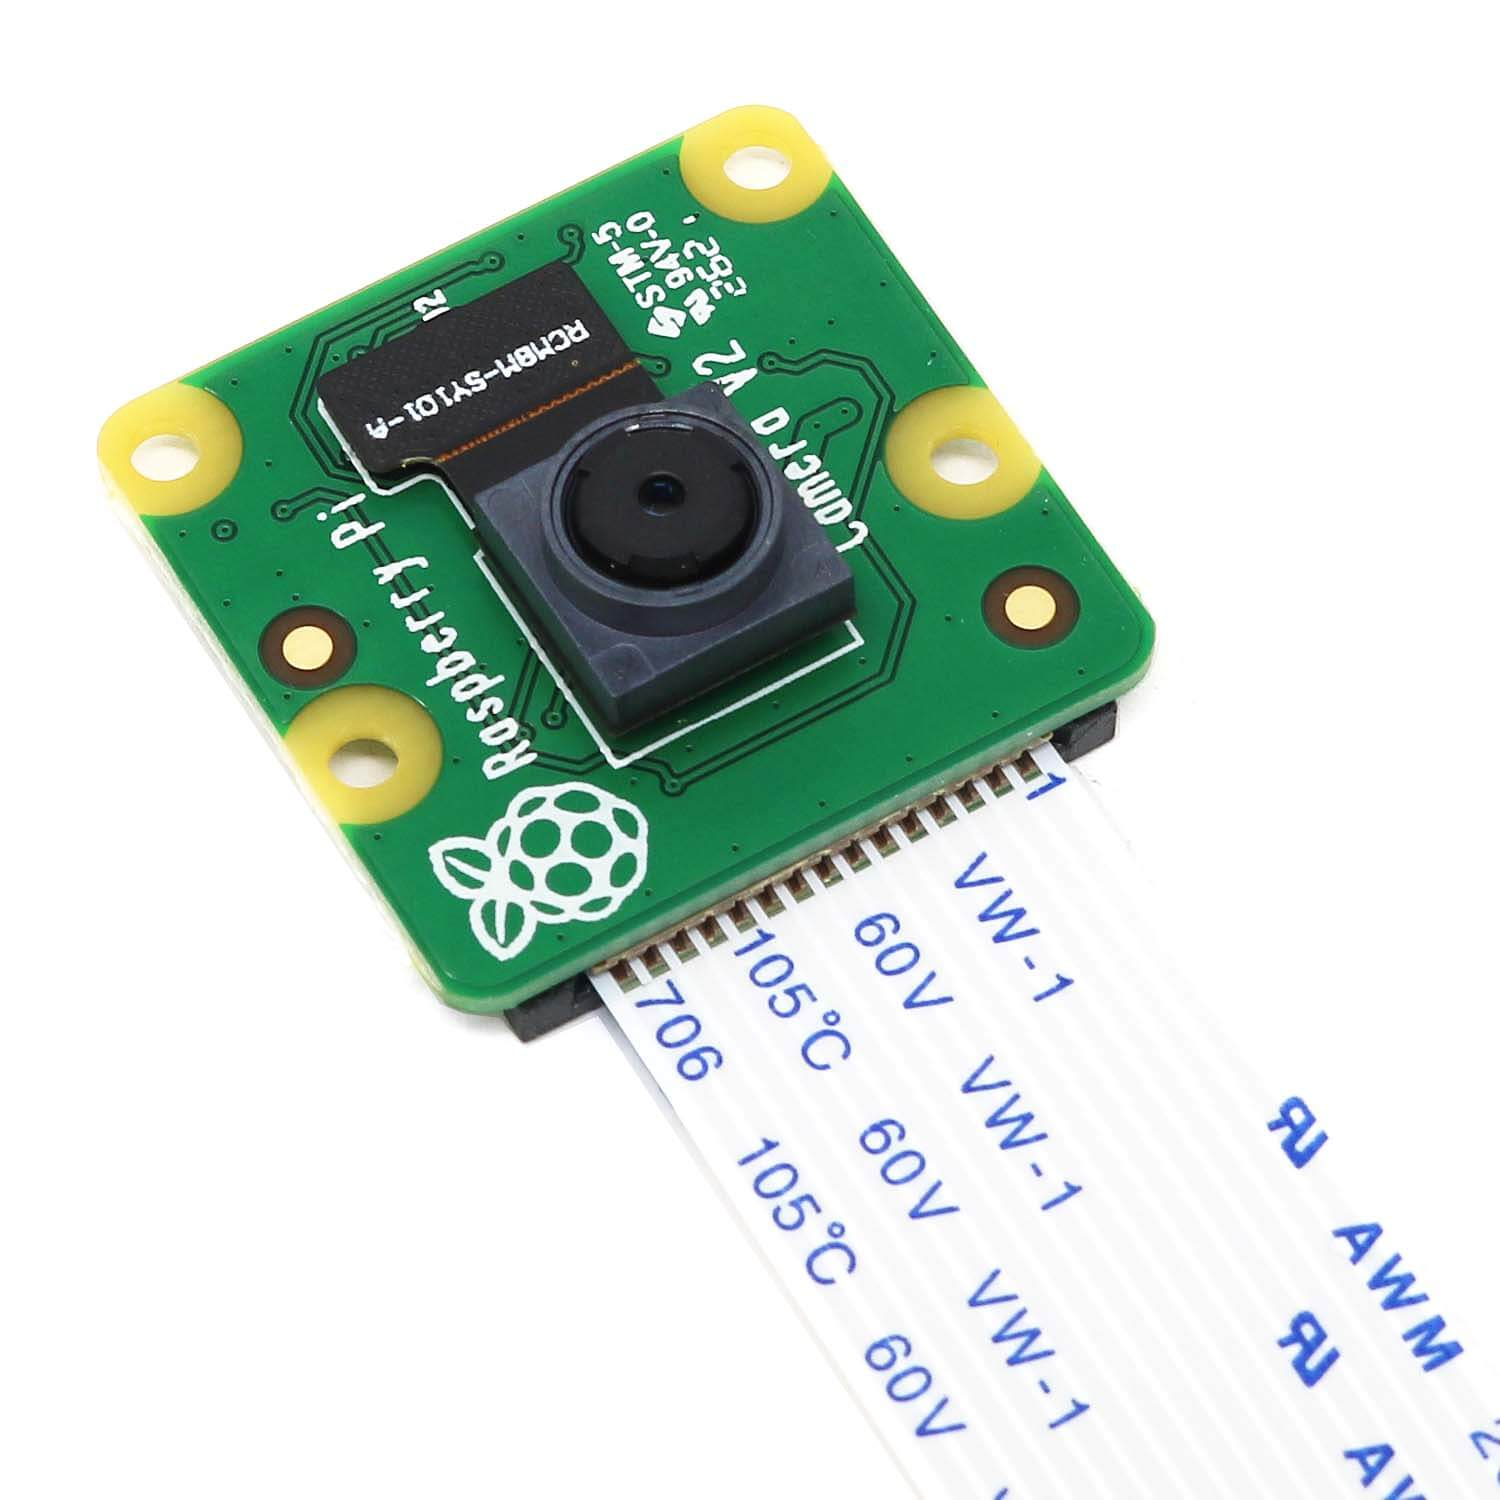
\includegraphics[width=4cm]{figs/picamera}
	\end{center}
	\caption{\textit{PiCamera} usada en la placa \textit{Raspberry Pi}.}
	\label{fig:picamera}
\end{figure}\

Un ejemplo de \textit{FIR} es \textit{BMW's FIR-based Autoliv Night Vision System} \cite{nightvision} (Figura \ref{fig:nightvision}), que trabaja con imágenes de 320 por 240 píxeles y cuenta con un rango de 300 metros. Este sistema utiliza lentes de gran angular que le permiten percibir la imagen con un mayor ángulo de visión.\\

\begin{figure} [h!]
	\begin{center}
		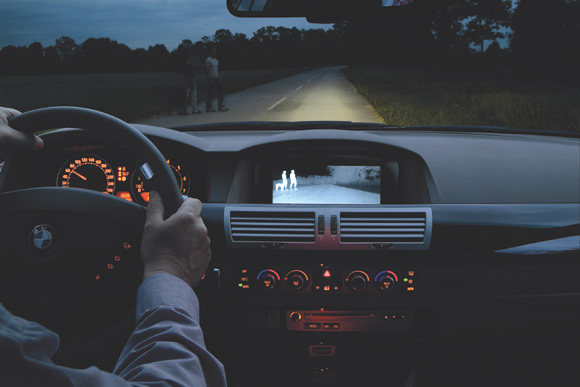
\includegraphics[width=8cm]{figs/nightvision}
	\end{center}
	\caption{Sistema de visión nocturna desarrollado por \textit{BMW}.}
	\label{fig:nightvision}
\end{figure}\

Una información de la imagen que puede resultar de interés es la distancia a la que se encuentra un objeto en concreto. Para calcularla, existen diversas soluciones. Por ejemplo, encontramos una solución con una única cámara, basada en la suposición de que todos los objetos se encuentran situados en el suelo en \cite{vega19d} o \cite{distanceopencv}. Para eliminar esta restricción y poder conocer distancias de objetos que no se encuentran situados en el suelo surgen las \textit{cámaras RGBD}, en las que cada píxel de la imagen proporciona, además del color RGB, una tercera componente, la profundidad o \textit{depth}. Una de las primeras cámaras \textit{RGBD} comerciales es la \textit{Kinect}, desarrollada por \textit{Microsoft} para su consola \textit{Xbox 360} (Figura \ref{fig:kinect}).\\

\begin{figure} [h!]
	\begin{center}
		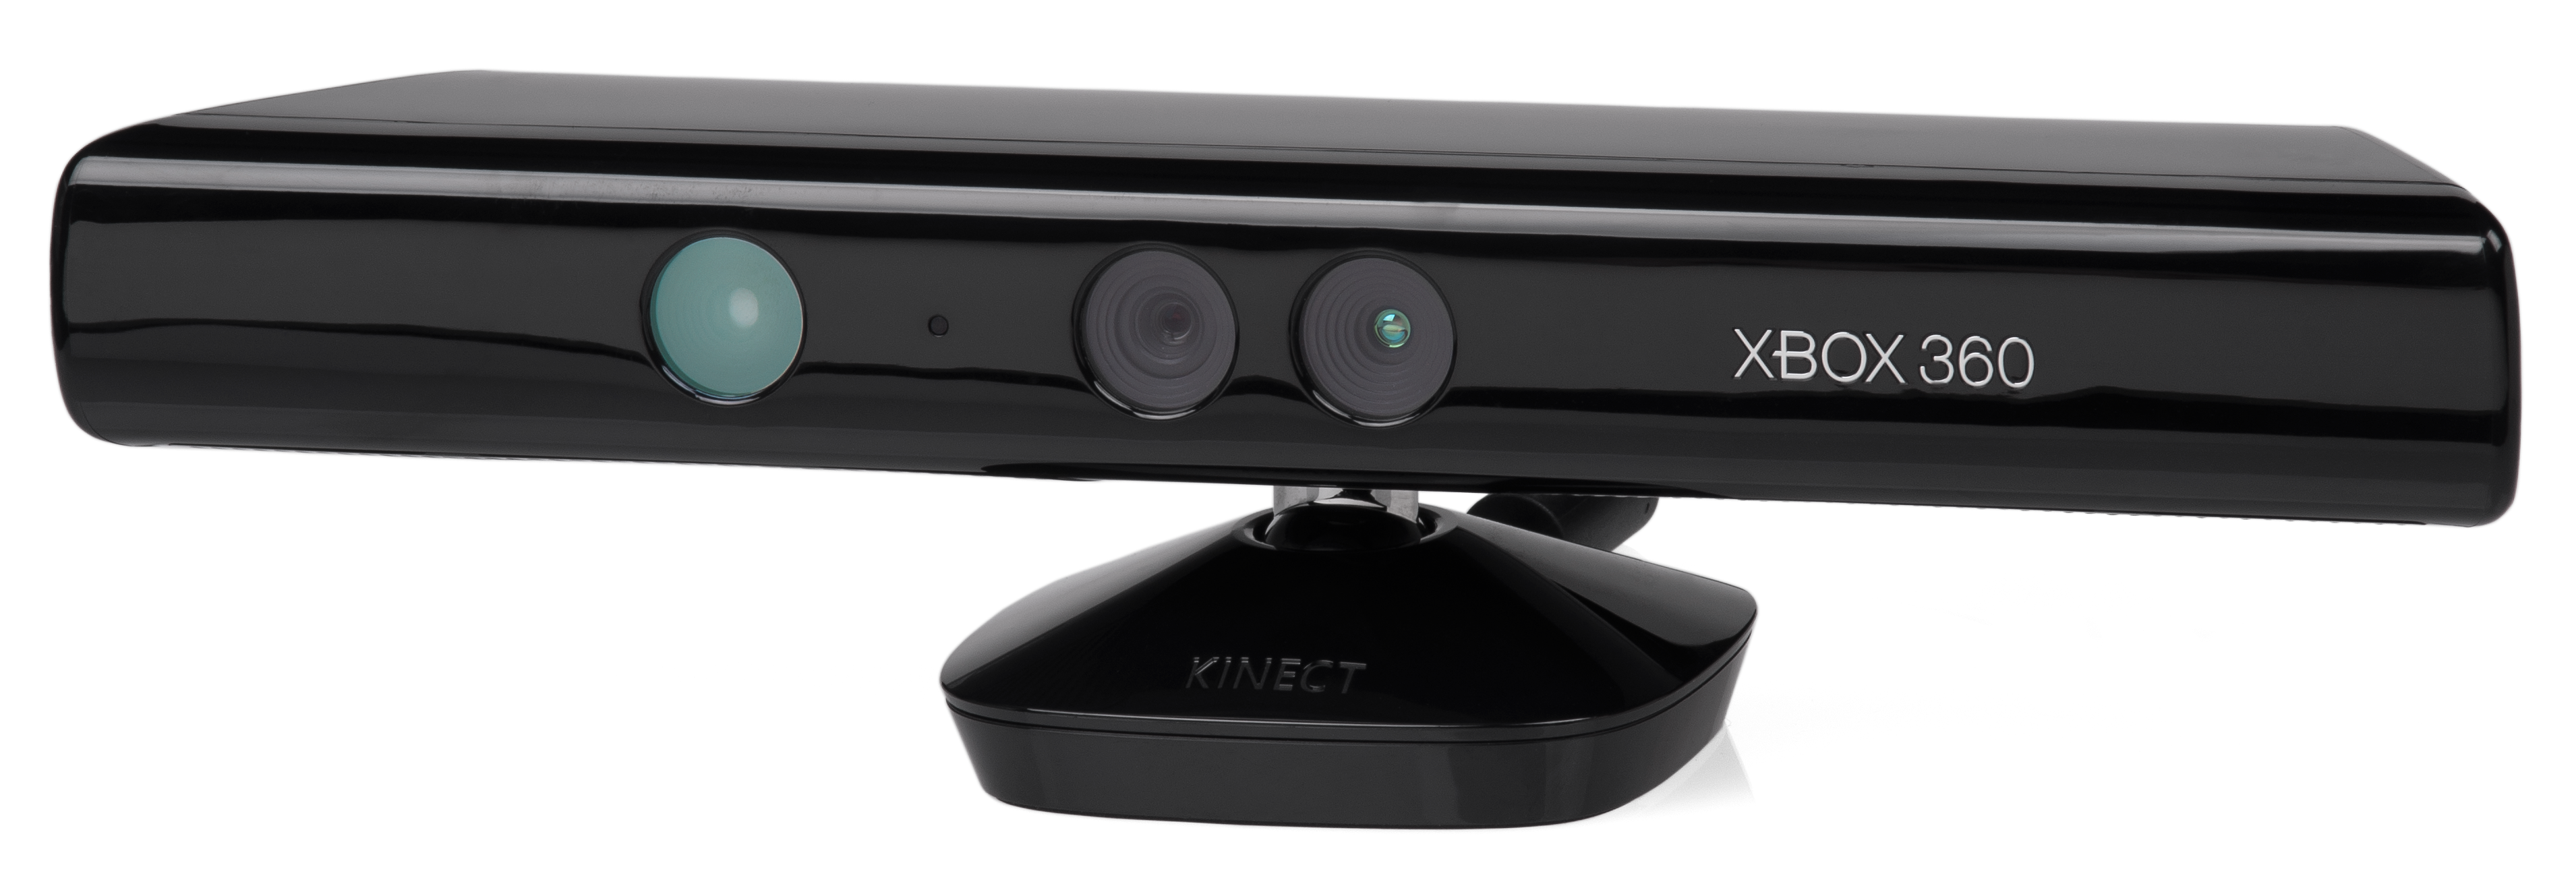
\includegraphics[width=6cm]{figs/kinect}\hspace{0.5cm}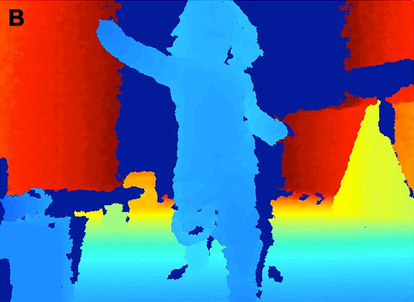
\includegraphics[width=6cm]{figs/depth}
	\end{center}
	\caption{Cámara \textit{RGBD Microsoft Kinect} e imagen de profundidad obtenida por esta.}
	\label{fig:kinect}
\end{figure}\

La visión artificial ofrece multitud de posibilidades, más allá de la robótica, ofrece numerosas aplicaciones en campos tan dispares como la medicina, la realidad aumentada, el procesamiento de señales o la agricultura.\\

\section{Deep Learning}
\label{sec:deeplearning}
El Aprendizaje Profundo, se basa en el uso de redes neuronales artificiales (o {\textit{Artificial Neural Network}}, (\textit{ANN})) que parten del aprendizaje automático, \textit{Machine Learning} que a su vez surge de la Inteligencia Artificial, \textit{Artificial Intelligence} (\textit{AI}). Las red neuronales está inspiradas en el cerebro humano donde una neurona se comunica con otra mediante señales. En el caso de su abstracción al mundo de la computación, una red está formada por una capa de entrada, una o más capas internas y una capa de salida (Figura \ref{fig:neuralnetwork}\footnote{\url{https://www.ibm.com/cloud/learn/neural-networks}}). Estas redes neuronales necesitan ser entrenadas mediante el concepto anteriormente introducido, de \textit{dataset}. A partir de este entrenamiento, la red es capaz de aprender y aumentar su precisión para que el resultado obtenido tenga fiabilidad.\\

\begin{figure} [h!]
	\begin{center}
		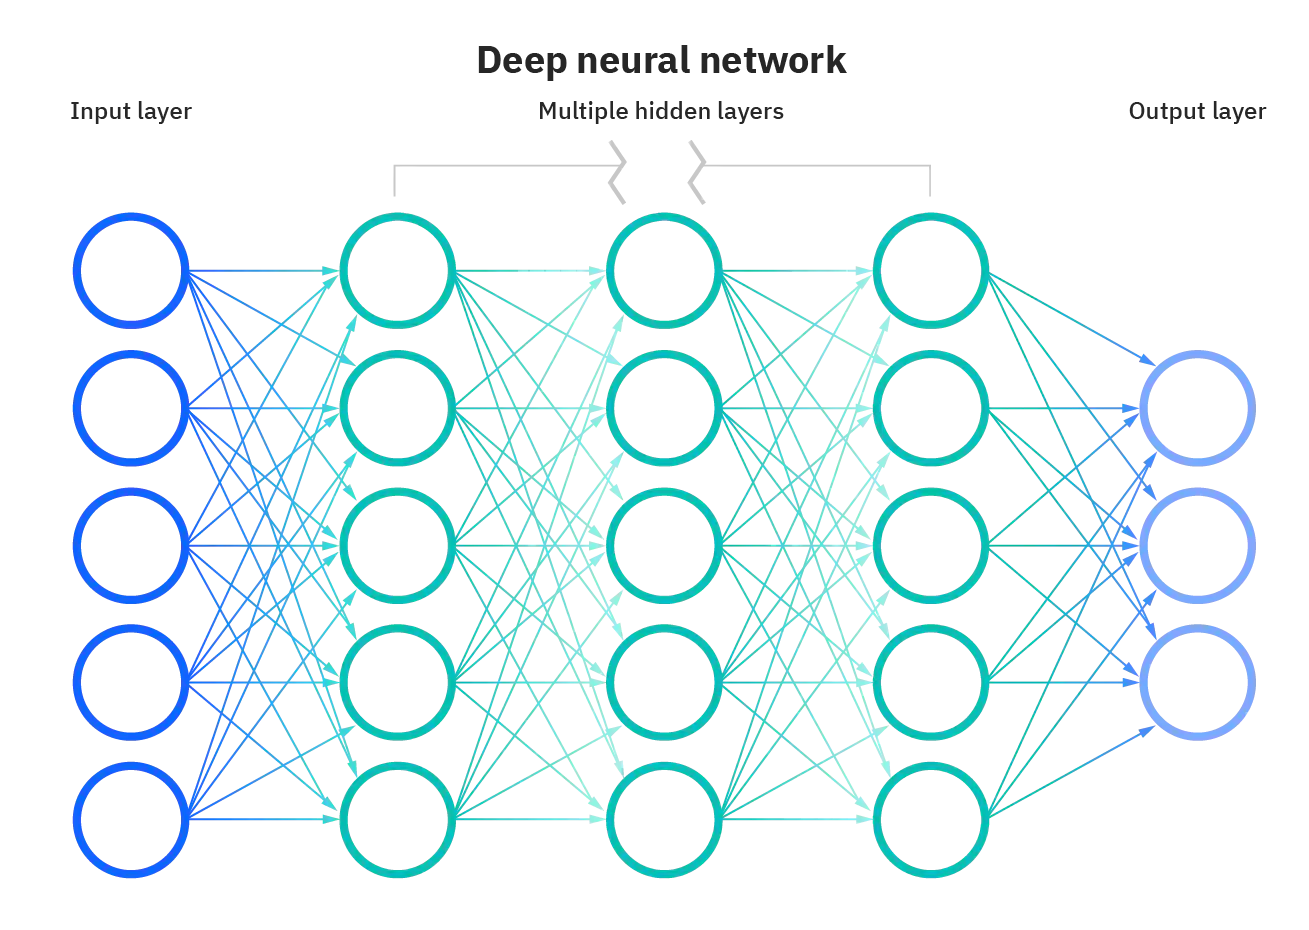
\includegraphics[width=10cm]{figs/neuralnetwork}
	\end{center}
	\caption{Red neuronal con tres capas internas.}
	\label{fig:neuralnetwork}
\end{figure}\

Los inicios del \textit{Deep Learning} se remontan al año 1979 cuando \textit{Kunihiko Fukushima} desarrolló una red neuronal de entre 5 y 6 capas llamada \textit{neocognitrón}\cite{neocognitron}, con el objetivo de reconocer caracteres japoneses.\\

Este tipo de redes neuronales tiene multitud de aplicaciones, pero todas comparten grandes cantidades de datos, en cualquier formato; vídeo, imagen, sonido. Algunas de ellas son: clasificación de objetos, procesamiento natural del lenguaje, \textit{Big Data}, análisis médico, conversión de imágenes en blanco y negro a color etc...\\

\section{Coches autónomos}
\label{sec:cochesautonomos}
Cuando pensamos en un vehículo autónomo, pensamos en vehículos que circulan a diario por las ciudades (coches, autobuses, furgonetas) aunque cabría esperar que sin una persona al volante. Pero a día de hoy, todavía no está presente en las ciudades pero cabe esperar que en un corto plazo de tiempo lo estará, el principal inconveniente que actualmente está frenando su implantación es la legislación, a diferencia de, por ejemplo, el entorno de la aviación, donde desde hace décadas el control de la aeronave es automático a excepción de tareas como el despegue, el aterrizaje o situaciones de emergencia.\\

Actualmente, coches de última generación como \textit{Tesla} (Figura \ref{fig:teslaobjectdetection}), ya incorporan un grado de autonomía elevado en determinadas situaciones, pero siempre con un conductor al volante que debe permanecer atento para poder reaccionar.\\

\begin{figure} [h!]
	\begin{center}
		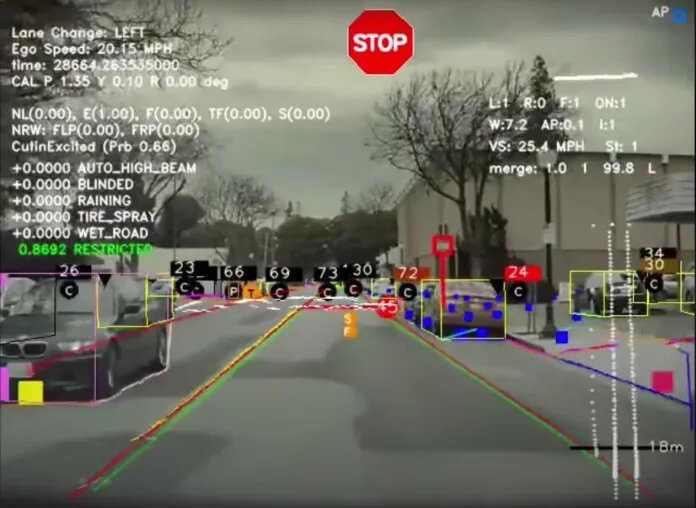
\includegraphics[width=12cm]{figs/teslaobjectdetection}
	\end{center}
	\caption{Sistema de conducción autónoma \textit{Tesla AutoPilot}.}
	\label{fig:teslaobjectdetection}
\end{figure}\

Atendiendo al estándar \textit{SAE J3016} \cite{saej3016} los niveles de autonomía se pueden dividir en cinco:
\begin{enumerate}
	\item Sin automatización: avisos y asistencia puntualmente.
	\item Asistencia a la conducción: centrado de carril o control de crucero.
	\item Automatización parcial: centrado de carril y control de crucero.
	\item Automatización condicionada: conducción automática en atascos.
	\item Automatización elevada: conducción automática en algunas situaciones.
	\item Automatización completa: conducción automática en cualquier situación.
\end{enumerate}\

\subsection{AMRs}
\label{sec:amr}
Los robots móviles autónomos (o \textit{Autonomous Mobile Robot}, \textit{AMR}) son aquellos capaces de navegar por entornos dinámicos, conviviendo con humanos a su alrededor y sabiendo sobreponerse a situaciones para las que no habían sido programados explícitamente. Son los sucesores de los vehículos de guiado automático (o \textit{Automated Guided Vehicle}, \textit{AGV}), los cuales requieren una cierta infraestructura dependiendo del tipo de guiado, ya sea filo-guiados, a través de pintura o a través de cualquier otra técnica que haga que ese vehículo sólo pueda funcionar cuando se sabe la infraestructura previa que estará presente en el entorno de trabajo.\\

Por otro lados, estos \textit{AGVs} presentan muchas dificultades para relacionarse con obstáculos o humanos, donde ante un cambio pequeño del entorno, el robot se detendrá por seguridad. A diferencia de estos, los \textit{AMRs} son capaces de realizar multitud de tareas en entornos donde la infraestructura necesaria es casi nula, quitando alguna necesidad de conectividad. Salvo por esa excepción, son robots que pueden ser diseñados para navegar por cualquier tipo de ambiente.\\

Un ejemplo muy representativo de \textit{AMRs}, son los robots de \textit{Kiva Systems}\footnote{\url{https://www.aboutamazon.es/noticias/innovacion/los-robots-en-numeros-datos-y-cifras-sobre-los-robots-en-amazon}} (Figura \ref{fig:kivasystems}), empresa comprada por \textit{Amazon} en 2012\footnote{\url{https://www.eleconomista.es/tecnologia/noticias/3833220/03/12/Amazon-compra-la-empresa-robotica-Kyva-Systems-por-775-millones-de-dolares.html}} para automatizar sus almacenes en tareas de logística a nivel interno, maximizando la productividad y el almacenamiento, tanto en profundidad como en altura y minimizando el coste en personal.\\

\begin{figure} [h!]
	\begin{center}
		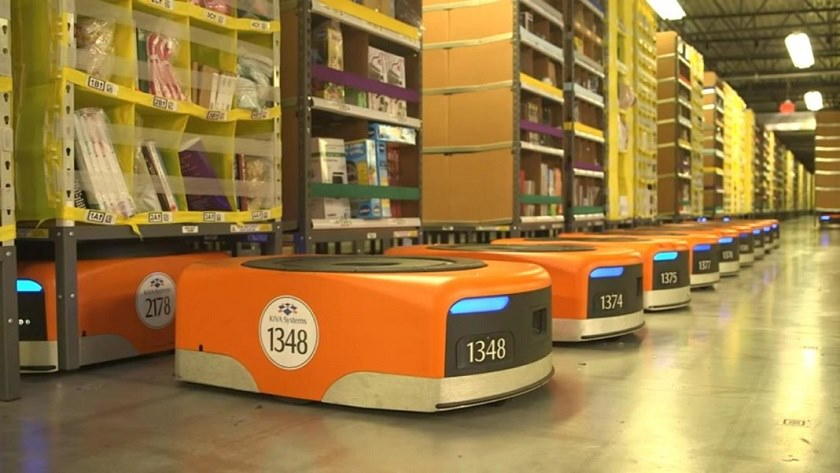
\includegraphics[width=8cm]{figs/kivasystems}
	\end{center}
	\caption{\textit{AMRs} de \textit{Kiva Systems} en almacenes de \textit{Amazon}.}
	\label{fig:kivasystems}
\end{figure}\

El presente trabajo se enmarca dentro del campo de la robótica y la visión artificial. En estas disciplinas se hace uso de todas estas tecnologías con el objetivo de dotar a robots de una cierta inteligencia. En los próximos capítulos se detallarán los objetivos a cumplir, las plataformas utilizadas y el diseño implementado.\\

%Mapa